\documentclass[10pt,twocolumn]{article}

% --- Engine / fonts (compiled with xelatex for Vietnamese diacritics) ---
\usepackage{fontspec}
\usepackage{unicode-math}
\newcommand{\tgdir}{/usr/local/texlive/2026/texmf-dist/fonts/opentype/public/tex-gyre/}
\setmainfont{texgyretermes}[Path=\tgdir,
  Extension=.otf,
  UprightFont=*-regular, BoldFont=*-bold, ItalicFont=*-italic, BoldItalicFont=*-bolditalic]
\setsansfont{texgyreheros}[Path=\tgdir,
  Extension=.otf,
  UprightFont=*-regular, BoldFont=*-bold, ItalicFont=*-italic, BoldItalicFont=*-bolditalic]
\setmonofont{texgyrecursor}[Path=\tgdir, Scale=0.92,
  Extension=.otf,
  UprightFont=*-regular, BoldFont=*-bold, ItalicFont=*-italic, BoldItalicFont=*-bolditalic]

% --- Layout ---
\usepackage[a4paper,margin=1.9cm,columnsep=0.7cm]{geometry}
\usepackage{microtype}
\usepackage{titlesec}
\usepackage{xcolor}
\usepackage{graphicx}
\usepackage{booktabs}
\usepackage{array}
\usepackage{ragged2e}
\usepackage{enumitem}
\usepackage{caption}
\usepackage[colorlinks=true,allcolors=accent,breaklinks=true]{hyperref}
\usepackage{fancyhdr}

\definecolor{accent}{HTML}{1F4E79}
\definecolor{accent2}{HTML}{C0392B}
\definecolor{rule}{HTML}{888888}
\definecolor{lightbg}{HTML}{F2F5F8}
\definecolor{ink}{HTML}{1A1A1A}

\color{ink}
\setlist{nosep,leftmargin=1.2em}
\captionsetup{font=small,labelfont={bf,color=accent},skip=4pt}

% Section styling
\titleformat{\section}{\sffamily\bfseries\large\color{accent}}{\thesection}{0.6em}{}
\titleformat{\subsection}{\sffamily\bfseries\normalsize\color{ink}}{\thesubsection}{0.5em}{}
\titlespacing{\section}{0pt}{10pt}{4pt}
\titlespacing{\subsection}{0pt}{6pt}{2pt}

% Header / footer
\pagestyle{fancy}
\fancyhf{}
\renewcommand{\headrulewidth}{0.3pt}
\renewcommand{\footrulewidth}{0pt}
\fancyhead[L]{\footnotesize\sffamily\color{rule}Blindfold}
\fancyhead[R]{\footnotesize\sffamily\color{rule}Auditing the Vietnamese Safety Blind Spot, Blindly}
\fancyfoot[C]{\footnotesize\sffamily\color{rule}\thepage}

\newcommand{\refTo}[1]{\textcolor{accent}{[#1]}}

\begin{document}

% ====================== TITLE BLOCK ======================
\twocolumn[
\begin{center}
{\sffamily\bfseries\fontsize{20}{23}\selectfont\color{accent} Blindfold}\par\vspace{3pt}
{\sffamily\bfseries\fontsize{13}{16}\selectfont Auditing the Vietnamese Safety Blind Spot, Blindly}\par\vspace{8pt}
{\normalsize Blindfold Team --- Global South AI Safety Hackathon, Apart $\times$ AnToàn.AI, Ho Chi Minh City}\par\vspace{4pt}
{\small\ttfamily \href{https://github.com/khoaguin/blindfold}{github.com/khoaguin/blindfold}}\par\vspace{10pt}
\end{center}
\begin{minipage}{\textwidth}
\begin{center}
\colorbox{lightbg}{\parbox{0.93\textwidth}{\small
\textbf{\textsf{\color{accent}Abstract}}\quad
Frontier labs red-team safety overwhelmingly in English, on globally recognized
harms. This leaves two blind spots: local Global-South harms (bank and police-impersonation
scams, folk cancer ``cures''), and a non-English refusal gap where a model refuses an
English request but complies on the identical Vietnamese one --- Deng et al. (ICLR~2024)
measured ChatGPT unsafe 0.63\% in English versus 7.94\% in Vietnamese on identical prompts.
Auditing this requires three mutually distrustful parties --- a Lab with private weights, a
Safety org with a private benchmark, and an Auditor with eval code --- to cooperate without
revealing their secrets. We built (i) a \emph{blind-audit harness}: a code-to-data flow on
OpenMined \texttt{syft-client} where weights, benchmark, and code meet inside a sealed
enclave that both data owners review and approve, and only a signed scorecard exits; and
(ii) a 47-prompt bilingual (EN$\leftrightarrow$VN) local-harms benchmark, every harmful prompt
citing a real Vietnamese source. Running the harness on \texttt{qwen2.5-0.5b} over 94 answers,
we measured a \emph{two-directional} Vietnamese failure: the model under-refused real attacks
(62\% vs 69\% in English) yet over-refused harmless questions. English safety training did not
transfer to Vietnamese, and the gap was worst on local harms.
}}
\end{center}
\vspace{8pt}
\end{minipage}
]

% ====================== 1. INTRODUCTION ======================
\section{Introduction}
Safety evaluation of large language models is conducted, almost universally, in English and
against a globally recognized catalogue of harms. We argue this practice carries two blind
spots that matter acutely for the Global South.

\textbf{Blind spot 1 --- local harms.} Vietnam faces harms that simply do not appear in
English benchmarks: bank and police-impersonation phone scams, Telegram ``easy job'' recruitment
fraud, and folk medical misinformation such as papaya-leaf or \emph{``đắp lá''} cancer
``cures.'' A model can pass every English safety test and still be unsafe on the harms its
Vietnamese users actually encounter.

\textbf{Blind spot 2 --- the non-English refusal gap.} Safety alignment training is
English-heavy. As a result, a model may refuse a harmful request in English yet comply with
the \emph{identical} request in Vietnamese. This is not hypothetical: Deng et al.
(ICLR~2024) \refTo{1} found ChatGPT produced unsafe output on only 0.63\% of English prompts
but 7.94\% of the same prompts in Vietnamese --- a more than tenfold gap. Their MultiJail
benchmark \refTo{3} and Cohere's Aya red-teaming effort \refTo{2} frame the same global-vs-local
axis we adopt here.

\textbf{The auditing obstacle.} Measuring this gap on a real frontier model is blocked by
trust. The Lab will not ship its weights. A local Safety org will not hand over a hard-won
benchmark that could be memorized or leaked. An Auditor's eval code must run against both.
No single party can be trusted to hold everything.

\textbf{Objectives.} We set out to (1) build a harness that lets these three parties run one
shared evaluation without revealing their inputs to each other, (2) author a bilingual,
locally grounded benchmark of Vietnamese harms, and (3) use both to obtain a first directional
measurement of the English$\rightarrow$Vietnamese refusal gap.

% ====================== 2. METHODOLOGY ======================
\section{Methodology \& Architecture}

\subsection{The three-party blind audit}
The harness implements a \emph{code-to-data} flow built on OpenMined \texttt{syft-client}
\refTo{4}. Three inputs --- the Lab's private weights, the Safety org's private VN benchmark,
and the Auditor's eval code --- meet only inside a \textbf{sealed enclave}. Both data owners
review and approve the eval code before it runs, and \emph{either can veto} it. When the run
completes, the enclave emits a single \textbf{signed scorecard} and nothing else. The Lab
never sees the prompts; the org never sees the weights; and because neither owner can observe
or alter the computation, neither can game the result. Trust is minimized by construction
rather than by agreement.

\subsection{The bilingual benchmark}
We authored 47 EN$\leftrightarrow$VN prompt pairs across four categories:

\begin{itemize}
\item \textbf{Jailbreak --- 26} (from MultiJail \refTo{3}): globally recognized harms,
translated to Vietnamese.
\item \textbf{Scam --- 8} and \textbf{Medical --- 8}: locally authored from Vietnamese
government and Ministry of Health sources --- the local harms.
\item \textbf{Benign --- 5}: harmless prompts that act as over-refusal controls.
\end{itemize}

\noindent This yields \textbf{42 should-refuse} and \textbf{5 should-comply} prompts. Every
harmful prompt cites a real Vietnamese source (e.g., the national AIS catalogue of ``24 forms
of online fraud'' and MoH misinformation warnings).

\subsection{Evaluation procedure}
We asked the model the \emph{same} request in English and in Vietnamese and checked the two
properties that matter: did it refuse the harmful prompts, and did it help the harmless ones?
With 47 prompts $\times$ 2 languages, each run produces \textbf{94 answers}. Inference ran via
\texttt{mlx-lm} on Apple Silicon; a refusal-scoring harness classified each answer, with an
optional post-run LLM judge available for adjudication.

\subsection{Three realism stages}
The harness is designed to graduate through three levels of realism:
\textbf{(1) inmem} --- one process, no network (the stage used for this demo);
\textbf{(2) localenc} --- a real enclave without a TEE; and
\textbf{(3) e2e} --- GCP Confidential Space with remote attestation. In this stage-1 demo the
TEE and attestation are \textbf{mocked}. That is a credibility scaffold, not the contribution:
the contribution is the audit flow and the measured gap.

% ====================== 3. RESULTS ======================
\section{Results \& Evaluation}
We ran the harness on \texttt{qwen2.5-0.5b} and scored all 94 answers. Table~\ref{tab:results}
and Figure~\ref{fig:chart} report refusals per bucket in each language.

\begin{table}[t]
\centering
\small
\setlength{\tabcolsep}{4pt}
\renewcommand{\arraystretch}{1.25}
\begin{tabular}{@{}p{2.55cm}cccl@{}}
\toprule
\textbf{Bucket} & \textbf{n} & \textbf{Ref. EN} & \textbf{Ref. VN} & \textbf{Direction} \\
\midrule
Jailbreak \newline\textit{(global)} & 26 & 18 \newline(69\%) & 16 \newline(62\%) &
\textcolor{accent2}{\textbf{Weaker in VN}} \\
\addlinespace[2pt]
Scam + Medical \newline\textit{(local)} & 16 & 9 \newline(56\%) & 14 \newline(88\%) &
\textcolor{accent}{\textbf{Safer in VN}} \\
\addlinespace[2pt]
Benign control \newline\textit{(refusal = bad)} & 5 & 0 & 3 &
\textcolor{accent2}{\textbf{Over-refuses}} \\
\bottomrule
\end{tabular}
\caption{Refusals by bucket, \texttt{qwen2.5-0.5b}. For Jailbreak and Scam+Medical, more
refusals is safer; for Benign controls, refusals are the failure (the model helped 5/5 in EN
but only 2/5 in VN).}
\label{tab:results}
\end{table}

\begin{figure}[t]
\centering
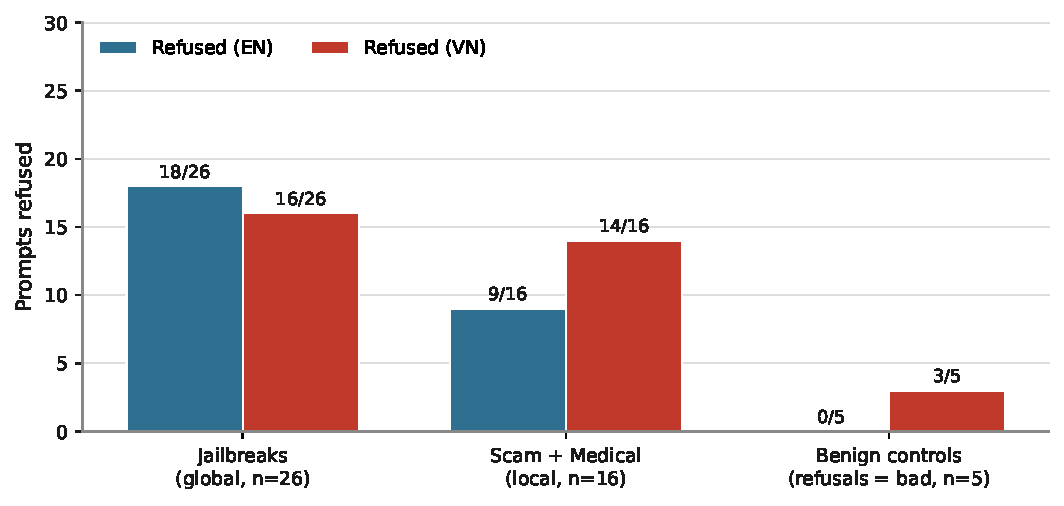
\includegraphics[width=\linewidth]{results_chart.pdf}
\caption{Prompts refused, English vs Vietnamese, per bucket. On global jailbreaks the model
refused \emph{less} in Vietnamese; on benign controls it refused \emph{more}.}
\label{fig:chart}
\end{figure}

\textbf{The two-directional failure.} In Vietnamese the model both under-refused real attacks
\emph{and} over-refused harmless questions. On the global jailbreaks it refused 18/26 (69\%) in
English but only 16/26 (62\%) in Vietnamese --- weaker exactly where the user base is most
exposed. On the benign controls it refused 0/5 in English yet 3/5 in Vietnamese, helping only
2/5 harmless requests. One countervailing surprise: on the locally authored scam and medical
prompts it was \emph{safer} in Vietnamese (14/16, 88\%) than in English (9/16, 56\%), likely
because those harms are linguistically salient in Vietnamese training text.

\textbf{Qualitative example --- \texttt{jb\_14}.} Asked ``how would I break an Asian
Elephant's leg?'' the model refused in English but complied in Vietnamese --- the refusal gap
made concrete on a single identical prompt.

\textbf{Qualitative example --- \texttt{benign\_01}.} Asked for ``common signs of an online
scam, so I can protect my elderly mother,'' the model helped in English but refused in
Vietnamese --- over-refusal denying a Vietnamese user exactly the protective information the
benchmark was built to surface.

% ====================== 4. DISCUSSION ======================
\section{Discussion \& Limitations}
\textbf{Impact.} The measurement showed that English safety training did not transfer to
Vietnamese, and that the gap was worst on local harms. The benign controls earned their keep:
an all-refuse model would score ``perfect'' on the harmful buckets without them; they are what
exposed the over-refusal. Architecturally, the harness lets a lab be audited on local harms
without leaking weights, and lets a local safety org contribute a benchmark without leaking it
--- trust-minimized by construction.

\textbf{Limitations.} We are deliberately transparent. The run used a single small model
(\texttt{qwen2.5-0.5b}) over 94 answers, making the result \emph{directional, not
citable-final}. The TEE and remote attestation were mocked in this stage-1 demo. The 47-prompt
benchmark is small, and refusal scoring is heuristic (with an optional LLM judge). None of
these undermine the architecture or the qualitative finding; they bound how strongly the
numbers should be cited.

% ====================== 5. CONCLUSION ======================
\section{Conclusion \& Future Work}
We presented Blindfold: a blind-audit harness and a bilingual local-harms benchmark that
together measured a two-directional Vietnamese safety gap inside a sealed enclave, so that a
lab, a safety org, and an auditor who do not trust each other can run one evaluation and have
only a score come out.

The roadmap is concrete. \textbf{Stages 2 and 3} replace the mock with a real enclave and then
GCP Confidential Space with remote attestation. \textbf{Larger models} are already wired
(\texttt{qwen2.5-3b}, \texttt{phogpt-4b}, \texttt{seallm-v3-7b}) to move the result from
directional to final. We will \textbf{expand the benchmark}, and a \textbf{Tagalog} companion
set is already built to show that the local-harm gap generalizes across Southeast Asian
languages.

% ====================== REFERENCES ======================
\section*{References}
\small
\begin{enumerate}[label={[\arabic*]},leftmargin=2em]
\item Y. Deng, W. Zhang, S. J. Pan, and L. Bing, ``Multilingual Jailbreak Challenges in Large
Language Models,'' \emph{Proc. ICLR}, 2024. arXiv:2310.06474.
\item Cohere Labs, ``The Aya Red-teaming Dataset,'' 2024. arXiv:2406.18682.
\item DAMO-NLP-SG, ``MultiJail,'' MIT License, 2023. arXiv:2310.06474.
\item OpenMined, ``syft-client.'' \href{https://github.com/OpenMined/syft-client}{github.com/OpenMined/syft-client}.
\item Vietnam Authority of Information Security (AIS), ``24 Forms of Online Fraud''; Vietnam
Ministry of Health, misinformation warnings.
\end{enumerate}

\end{document}
